\documentclass[12pt]{article}
\usepackage{setspace,palatino,multirow}
\usepackage{amsmath, amsfonts, amssymb, amsthm}
\usepackage{latexsym}
\usepackage{graphicx}
\usepackage{harvard}
\usepackage{longtable}
\usepackage{booktabs}
\usepackage{appendix}
\usepackage{listings}
\usepackage{dcolumn}

\usepackage{graphicx}
\usepackage{float}
\usepackage[usenames,dvipsnames]{color}
\usepackage[margin=1in]{geometry}
\usepackage{pdflscape}
\usepackage[flushleft]{threeparttable}
\usepackage[hang,flushmargin]{footmisc}
\usepackage{color}
\usepackage{indentfirst}
\usepackage{cite}

\usepackage[affil-it]{authblk} 
\usepackage{etoolbox}
\usepackage{lmodern}
\renewcommand{\qedsymbol}{$\blacksquare$}
\usepackage{amsthm,amssymb}
\usepackage{url} %Required
\usepackage{graphicx} %Required
\usepackage{array, booktabs, makecell}
\usepackage{siunitx, mhchem}
\usepackage{color}
\newcommand{\red}{\color{red}}
\newcommand{\blue}{\color{blue}}
\frenchspacing %Required
\setlength{\pdfpagewidth}{8.5in} %Required
\setlength{\pdfpageheight}{11in} %Required
\usepackage{multirow}
\usepackage[most]{tcolorbox}
\definecolor{block-gray}{gray}{0.9}
\newtcolorbox{myquote}{colback=block-gray,grow to right by=-0mm,grow to left by=-0mm, boxrule=0pt,boxsep=0pt,breakable}

% my lesson counter

\newcounter{lessoncounter}
\newcommand{\lesson}[1]{\refstepcounter{lessoncounter}\label{#1}}
\renewcommand{\qedsymbol}{\rule{0.7em}{0.7em}}

\makeatletter
\patchcmd{\@maketitle}{\LARGE \@title}{\fontsize{16}{19.2}\selectfont\@title}{}{}
\makeatother

\setlength{\parskip}{1em}
\renewcommand\Authfont{\fontsize{14}{14.4}\selectfont}
\renewcommand\Affilfont{\fontsize{12}{14.4}\selectfont}
\renewcommand{\baselinestretch}{1.3}
\usepackage[utf8]{inputenc}


\title{Overview of The Clean Coder}
\author{Akash Singh}
\affil{School of Computer Science, McGill University, Montreal, Canada}
\setcounter{MaxMatrixCols}{10}
% \doublespacing
\date{}
\begin{document}
\maketitle
% inline
{\Large \textbf{Clean Code}\par}


Have you ever been disrupted by bad code? If you are a programmer with any level of experience, you would have come across such situations. There is a name for it: \textit{wading}. Obviously, a working mess is better than nothing. Have you ever thought of this, "I will fix it later." :) [I am already feeling guilty!]

"Later equals never."

Bad coding practice leads to messy code. As the mess builds, the productivity of the team continues to decrease, asymptotically approaching zero. This leads to addition of more staff in the team in hopes of increasing productivity. But that new staff is not versed in the design of the system. They don’t know the difference between a change that matches the design intent and a change that thwarts the design intent. Furthermore, they, and everyone else on the team, are under horrific pressure to increase productivity. So they all make more and more messes, driving the productivity ever further toward zero.

Total cost owing a mess is huge and seldom leads to transformation of a functional application to a prototype. This leads to additional expenses in redeveloping the entire application. Alright, let's blame the managers for setting unrealistic deadlines, right? - No. Manager, marketers and the leadership team looks at us for the information they need to make promises and commitments. Its our job to tell them what we think about the proposed schedule. You might think of getting fired or setting a bad reputation, but tell me one manager that is ready to accept bad code just to meet the deadlines. No one is willing to take that risk as they know the challenges awaiting on deploying the code in the production environment or on scaling the application. If you set propose a feasible deadline, they will defend it with passion and vigour; its part and parcel of their job. Therefore, its our job to write the code with the same passion.
\begin{myquote}
\lesson{lesson:cleanCode}
\textbf{Lesson \ref{lesson:cleanCode}:} "All developers feel the pressure to make messes in order to meet deadlines. But they don’t take the time to go fast! The only way to make the deadline—the only way to go fast—is to keep the code as clean as possible at all times."
\end{myquote}
% \begin{proof}[Point to remember:]

% \end{proof}

\noindent \textbf{So, what is clean code?}
\begin{proof}[]
"I like my code to be elegant and efficient. The logic should be straightforward to make it hard for bugs to hide, the dependencies minimal to ease maintenance, error handling complete according to an articulated strategy, and performance close to optimal so as not to tempt people to make the code messy with unprincipled optimizations. Clean code does one thing well." - \textit{Bjarne Stroustrup (inventor C++)}
\end{proof}

This report will further discuss this in detail. It will start with naming convention to be used whilst coding followed by function identification in the code. Further, it will discuss the comment procedure, formatting and a bit about data structure selection. Finally, it will end with Formatting, Exception Handling and Unit Testing procedures to be followed to write a clean and maintainable code.

{\Large \textbf{Naming Conventions}\par}
We can follow some simple rules for creating good names:
\begin{enumerate}
    \item \textbf{Use intention-revealing names: }Choosing good names takes time but saves more time than it takes. For instance,
        \begin{figure*}[h]
         \centering
          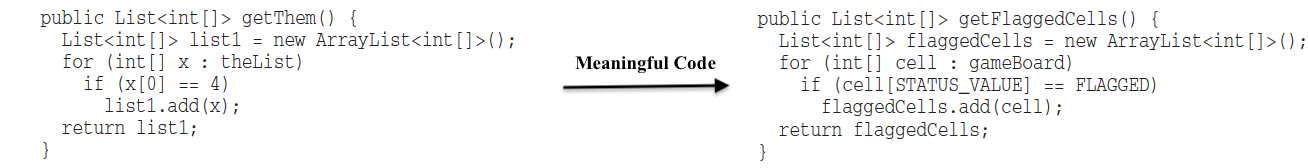
\includegraphics[width=0.9\textwidth]{CleanCodeImages/CleanCode.png}
         \caption{Exemplification of a meaningful code.}
         \label{fig:screenshot}
        \end{figure*}   
        
    \item \textbf{Avoid Disinformation: }Avoid leaving code that obscure the meaning of the code. For instance, hypotenuse and hp looks like a good abbreviation, it could be disinformative. Likewise, you cannot name a variable as accountList unless its actually a List, in such a case account/accountGroup will be better. Another awful case of disinformation is the use of the lower-case L or the upper-case O.
    
    \item \textbf{Make meaningful distinctions:} Don't write a code only to satisfy a compiler or an interpreter. For a compiler if the variable names are different then they mean different but its not the same for humans. For instance, the variable moneyAmount is indistinguishable from money for a human, get is same as retrieve, etc. Its best if we follow a uniform convention of variable naming. Note that there is nothing wrong with using prefix conventions like a and the so long as they make a meaningful distinction.
    
    \item \textbf{Use Pronounceable Names: } Consider an example: "private Date genymdhms". It represents (generation date, year, month, day, hour, minute, and second) so you will walk around saying “gen why emm dee aich emm ess”. It sounds silly, good for a short laugh. Right to write the same will be "private Date generationTimestamp;"
    
    \item \textbf{Avoid Encodings: }
    \begin{itemize}
        \item Member prefixes is not needed in most of the current tech-stack. For ex: if there is a member variable in java, there is no need to prefix that variable with \textit{m_}.
        \item There is no need to start an interface name with the letter \textit{I}.
        \item Avoid mental mapping, a very common example is the use of variable i, j, k for nested loops where we know the purpose of each variable but we don't put in the right effort to create a variable name accordingly. This is a must.

    \end{itemize}
    \item \textbf{Class names:} Classes and objects should have a noun or a noun phrase. Eg: Customer, WikiPage, etc. Avoid using verbs like Data, Info, Manager, etc.
    
    \item \textbf{Method names: }Methods should have verb or verb phrase names like postPayment, deletePage, or save. Accessors, mutators, and predicates should be named for their value and prefixed with get, set, etc.    
    \item \textbf{Don't be cute: }Cuteness in code often appears in the form of jargon or slang. For example, don’t use the name whack() to mean kill() or eatMyShorts() to mean abort().
    \item \textbf{Pick one word per concept: }For instance, it’s confusing to have \textif{fetch, retrieve, and get} as equivalent methods of different classes. Likewise, it’s confusing to have a \textit{controller and a manager and a driver} in the same code base.
    
    \item \textbf{Distinguish when to use a solution based name and when to use a problem specific name: }Remember that the people who read your code will be programmers. So go ahead and use computer science (CS) terms, algorithm names, pattern names, math terms, and so forth. There are lots of very technical things that programmers have to do. Choosing technical names for those things is usually the most appropriate course. Separating solution and problem domain concepts is part of the job of a good programmer and designer. The code that has more to do with problem domain concepts should have names drawn from the problem domain.
\end{enumerate}


\end{document}